\cleardoublepage%
\chapter*{\label{chap:apx_e}Appendix E - Code and Experimental Data\chaptermark{Appendix E}}%
\chaptermark{Appendix E}%
\addcontentsline{toc}{section}{Appendix E - Code and Experimental Data}

\section*{Maximum Range Test and Reliability and Robustness Test Code}
\addcontentsline{toc}{subsection}{Maximum Range Test and Reliability and Robustness Test Code}
\subsection*{boop-o-meter Code:}
[...]
%\lstinputlisting[breaklines]{./software/applications/boop-o-meters/boop-o-meter 300.py}
% \subsection*{Results:}

% During the robustness test, no outages of devices was observed when sending out messages with 19 devices at the same time. \\\\
% With regards to the maximum range test, the longest distance at which messages could still be sent and received by both devices was 242 meters as shown in Figure \ref{fig:range}

% \begin{figure}
%     \centering
%     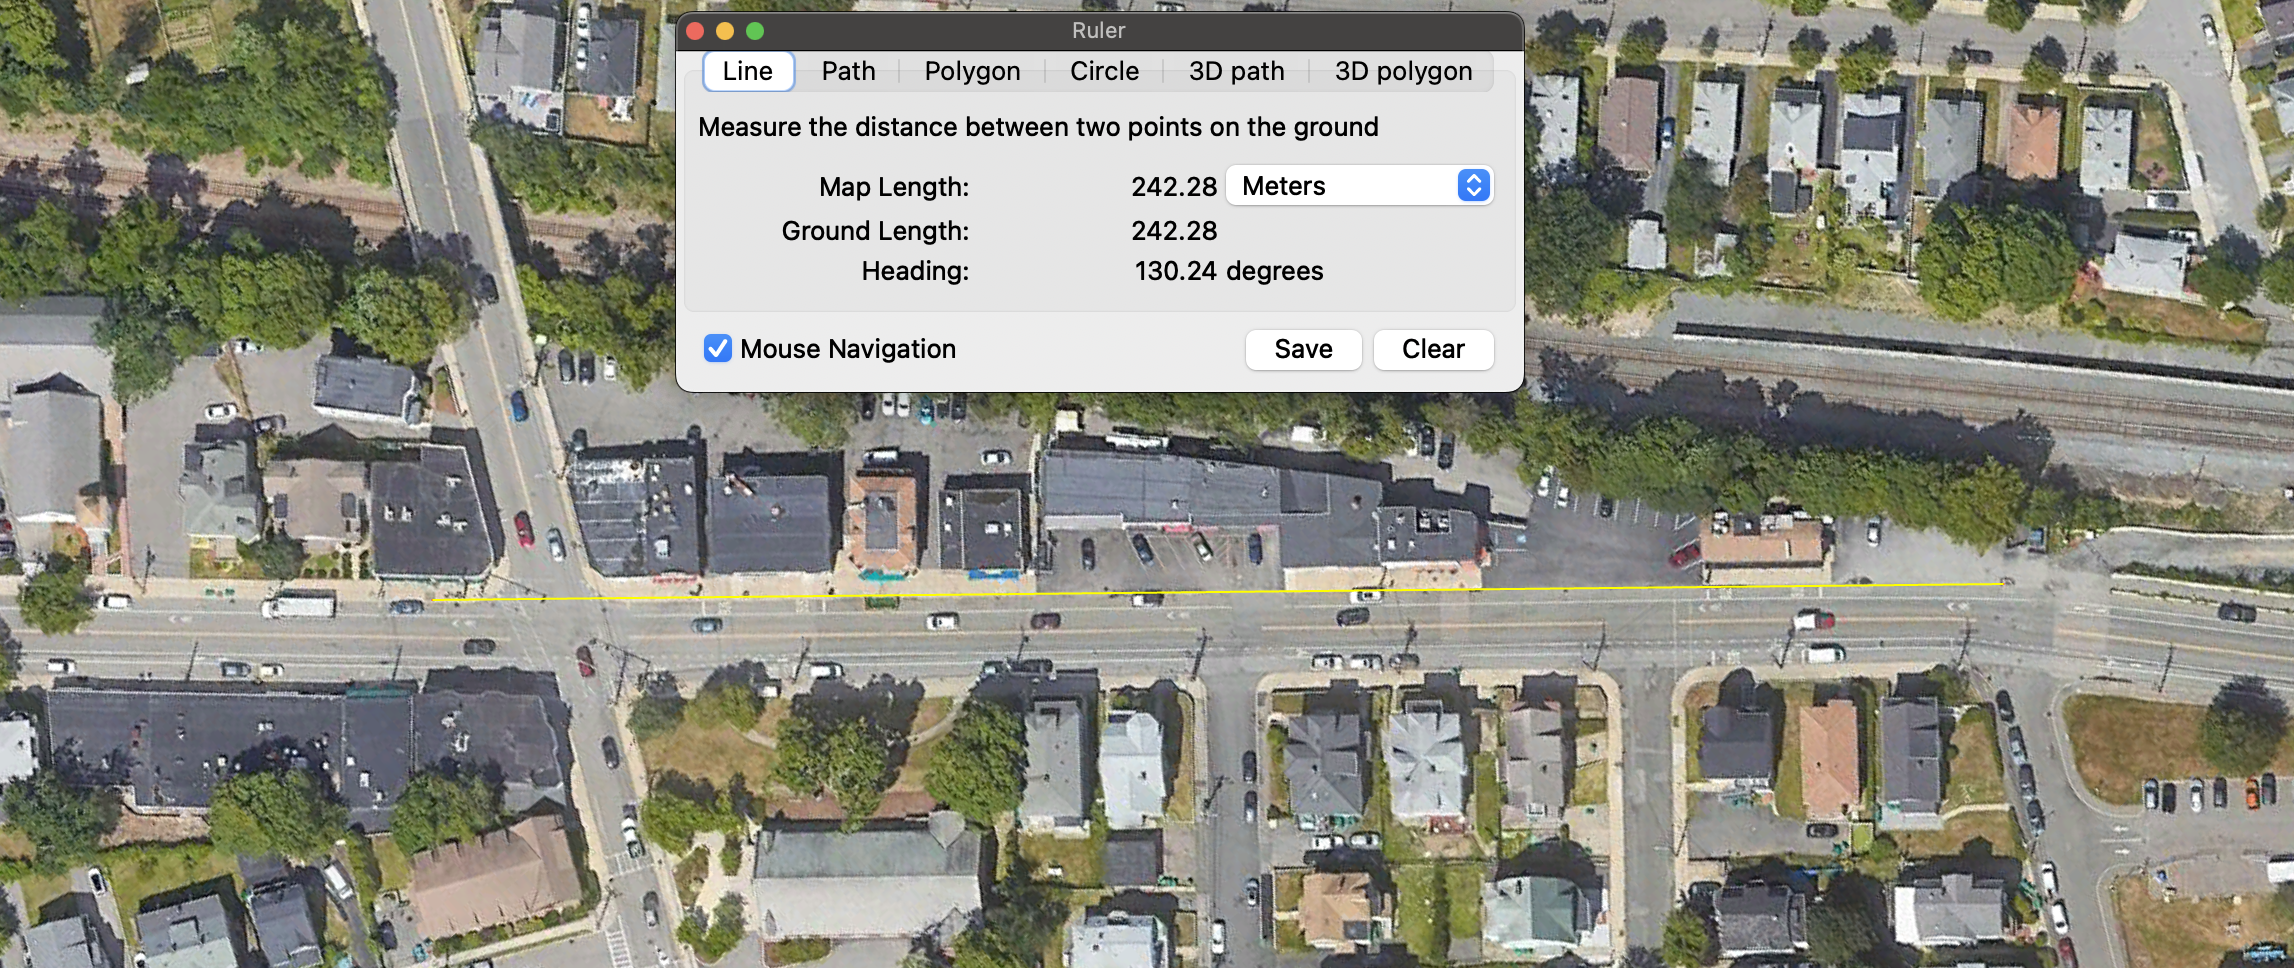
\includegraphics[width=\linewidth]{overleaf/images/range.png}
%     \vspace{\ftspace}
%     \caption{Maximum message transmission range}
%     \label{fig:apx:range}
% \end{figure}

\section*{Ping Response Time}
\addcontentsline{toc}{subsection}{Ping Response Time}
\subsection*{Code:}
\subsubsection*{Shout:}
[...]
%\lstinputlisting[breaklines]{./software/applications/ping/shout.py}
\subsubsection*{Echo:}
[...]
%\lstinputlisting[breaklines]{./software/applications/ping/echo.py}
% \subsection*{Results:}
% \begin{table}[H]
%     \centering
%     \begin{tabular}{c|c}
%          &  \\
%          & 
%     \end{tabular}
%     \vspace{\ftspace}
%     \caption{Caption}
%     \label{tab:apx:ping_results}
% \end{table}

\section*{Response Time, RSSI and Packet Loss Rate Depending on Range Test Code}
\addcontentsline{toc}{subsection}{Response Time, RSSI and Packet Loss Rate Depending on Range Test Code}
\subsection*{Code:}
[...]
%\lstinputlisting[breaklines]{./software/applications/rssi_testing/rssi.py}
% \subsection*{Results:}
% \begin{table}[H]
%     \centering
%     \begin{tabular}{c|c}
%          &  \\
%          & 
%     \end{tabular}
%     \vspace{\ftspace}
%     \caption{Caption}
%     \label{tab:apx:rssi_results}
% \end{table}

\section*{Battery Consumption}
\addcontentsline{toc}{subsection}{Battery Consumption}
\subsection*{Code:}
[...]
%\lstinputlisting[breaklines]{./software/applications/rssi_testing/rssi.py}
%\subsection*{Results:}
%...